\section{Controllo decentralizzato a giunti indipendenti \\ {\small \textit{Decentralized Joint Space Control}}}

Nel controllo decentralizzato a giunti indipendenti \textbf{ogni} singolo \textbf{giunto} attuato è considerato come un \textbf{sottosistema SISO disaccoppiato e indipendente}, descritto da un modello dinamico approssimato. Gli \textbf{effetti di accoppiamento} non-lineari presenti nella dinamica propria del robot sono \textbf{considerati come disturbi}.

Lo schema di controllo complessivo è formato da $n$ controllori (uno per ogni giunto), basati su reti di compensazione classiche, ciascuno agente in modo indipendente dagli altri.\\
Ricordiamo che il nostro obiettivo è quello di far eseguire una sequenza $\mathbf{q}(t)$ in modo che $\mathbf{q}(t) \to \mathbf{q}_d(t)$.\\	


\begin{figure}[th!]
	\centering
	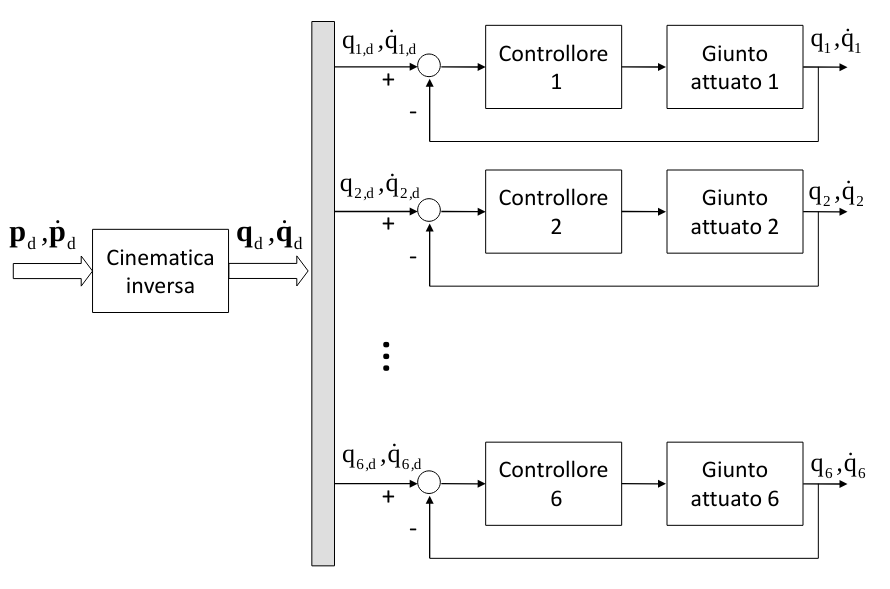
\includegraphics[width=0.7\linewidth]{images/decentralized_joint_space_control_1}
	\caption{Schema generale del controllo a giunti indipendenti}
	\label{fig:decentralizedjointspacecontrol1}
\end{figure}


Come accennato in precedenza, in questo caso andremo a controllare gli attuatori in velocità. È possibile dimostrare (vedi dopo) la seguente assunzione:
$$
\mathbf{G}_v\mathbf{v}_c \approx \mathbf{K}_\omega\mathbf{K}_r\mathbf{\dot{q}}
$$
L'importante di questa espressione è la proporzionalità fra $\mathbf{G}_v$ e  $\dot{\mathbf{q}}$ (velocità), che notiamo essere indipendente dai parametri del manipolatore. Inoltre questa proporzione è tanto più valida quanto velocità/accellerazioni sono piccole (per questa cosa viene in aiuto anche il gear-reduction ratio).

\begin{mdframed}[leftmargin=15pt, rightmargin=15pt, leftline=false, rightline=false]
\textit{Dim.}

\textit{
Partendo dal modello dinamico {\boldmath$B(q)\ddot{q} + C(q, \dot{q})\dot{q} + F_v\dot{q} + g(q) = \tau$} introduciamo in esso la frizione viscosa elettrica. Ovvero poniamo {\boldmath$F_v = F_\text{v. mech.} + F_\text{v. electr.} = F_\text{v. mech.} + K_rK_tR_a^{-1}K_\omega K_r$}. \\
Inoltre dal modello del motore: 
{\boldmath$\tau_m = K_r^{-1} \tau = K_t I_a \implies \tau = K_r K_t I_a$}. Sappiamo anche che $V = Ri \implies i = \frac{V}{R}$ e quindi, ricordando che {\boldmath$V_c = G_v V_c^{'}$}, otteniamo {\boldmath $I_a = R_a^{-1}G_v V_c$}. Unendo il tutto otteniamo {\boldmath $\tau = K_r K_t R_a^{-1}G_v V_c$}.\\
Inserendo tutto nella formula del modello dinamico otteniamo:
\boldmath
$$
B(q)\ddot{q} + C(q, \dot{q})\dot{q} + F_{\text{v. mech.}}\dot{q} + g(q) = K_r K_t R_a^{-1}G_v V_c - K_rK_tR_a^{-1}K_\omega K_r
$$
Ovvero, raccogliendo i termini a destra (ricordando che originalmente quello era $\tau$):
\begin{equation}\label{eq:torque_command}
\tau =  K_r K_t R_a^{-1}(G_v V_c - K_\omega K_r \dot{q})
\end{equation}
Quello che otteniamo fra le parentesi è l'espressione ipotizzata inizialmente.\\
(la quasi uguaglianza viene dal fatto che $K_r \gg 1$, $R_a$ molto piccolo, $\tau$ non troppo grosso).
}

\raggedleft $\square$
\end{mdframed}


\vspace*{25pt}



Richiamando i capitoli precedenti, ricordiamo che il modello dinamico del manipolatore in assenza di forze scambiate con l’ambiente esterno è espresso da:
\boldmath
\begin{equation}\label{eq:dynamic_no_ext_forces}
B(q)\ddot{q} + C(q, \dot{q})\dot{q} + F_v\dot{q} + g(q) = \tau = K_r \tau_m
\end{equation}
\unboldmath

L'ultima uguaglianza deriva dall'utilizzo dei motoriduttori (vedi (\ref{eq:trasmission_reduction_torque})).

Per elaborare uno schema di controllo decentralizzato ai giunti è opportuno riportare le equazioni dinamiche a monte del motoriduttore (sul primario, i.e. lato motore):
\boldmath
$$
K_r^{-1}B(q)K_r^{-1}\ddot{q}_m + K_r^{-1}C(q, \dot{q})K_r^{-1}\dot{q}_m + K_r^{-1}F_vK_r^{-1}\dot{q} + K_r^{-1}g(q) = \tau_m
$$
\unboldmath

(Questa equazione è ottenuta semplicemente applicando (\ref{eq:trasmission_reduction}) e (\ref{eq:trasmission_reduction_torque}) a (\ref{eq:dynamic_no_ext_forces})).

È possibile notare che $\mathbf{B}(q)$ può essere decomposto in $\mathbf{B}(q) = \bar{\mathbf{B}} + \Delta\mathbf{B}(q)$, ove $\bar{\mathbf{B}}$ è una matrice diagonale costante e $\Delta\mathbf{B}(q)$ è una matrice configuration-dependent. Possiamo quindi riscrivere l'ultima equazione come:
\boldmath
\begin{gather*}
(\bar{B} + \Delta B(q)) K_r^{-1} \ddot{q} + C(q, \dot{q})K_r^{-1}\dot{q} + F_vK_r^{-1}\dot{q} + g(q) = K_r \tau_m \\
\Downarrow \\
K_r^{-1}\bar{B}K_r^{-1}\ddot{q}_m + 
\underbrace{K_r^{-1}\Delta B(q)K_r^{-1}\ddot{q}_m + K_r^{-1}C(q, \dot{q})K_r^{-1}\dot{q}_m + K_r^{-1}g(q)}_{disturbances}
+ K_r^{-1}F_vK_r^{-1}\dot{q}_m  = \tau_m
\end{gather*}


E, come evidenziato nell'equazione, possiamo considerare gli effetti degli altri giunti su quello corrente come \textbf{disturbi}:
\begin{equation}\label{eq:dynamic_disturbances}
	d = K_r^{-1}\Delta B(q)K_r^{-1}\ddot{q}_m + K_r^{-1}C(q, \dot{q})K_r^{-1}\dot{q}_m + K_r^{-1}g(q)
\end{equation}

Inoltre, visto che questi termini sono moltiplicati per $\mathbf{K}_r^{-1}$, \textbf{più alto è il gear-ratio e meno questi termini influenzeranno il nostro sistema} ($d \downarrow$ quando $K_r \uparrow$), portandoci così ad un sistema sempre più lineare e disaccoppiato (ovviamente c'è un limite, visto che gear-ratio altissimi non produrrebbero praticamente alcune velocità).

Riassumendo:


\begin{equation}\label{eq:dynamic_with_disturbances}
K_r^{-1}\bar{B}K_r^{-1}\ddot{q}_m + F_m\dot{q}_m + d = \tau_m
\end{equation}
dove $F_m \triangleq K_r^{-1}F_vK_r^{-1}$. 
\unboldmath



\begin{figure}[t]
	\centering
	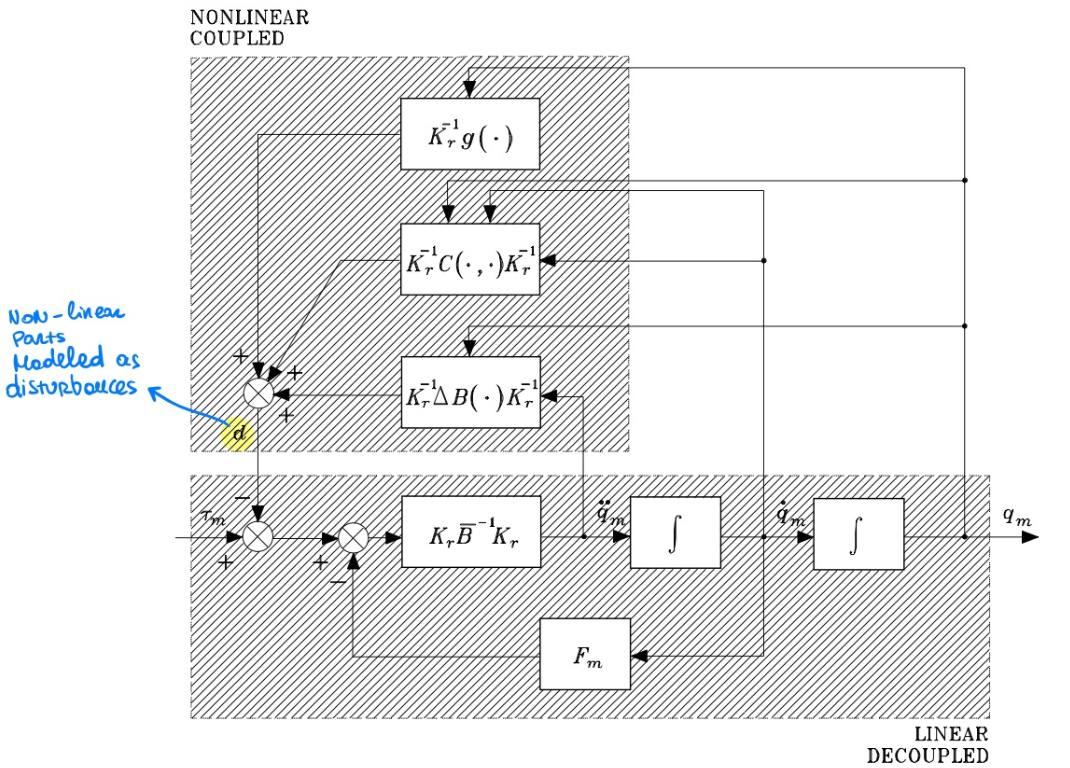
\includegraphics[width=0.7\linewidth]{images/decentralized_joint_space_control_2}
	\caption{Circuito relativo a (\ref{eq:dynamic_with_disturbances})}
	\label{fig:decentralizedjointspacecontrol2}
\end{figure}

Detto questo, per la parte lineare possiamo ora far riferimento alla nota teoria del controllo LTI per sistemi SISO.



\subsection{Controllo del singolo giunto}

Partendo da (\ref{eq:dynamic_with_disturbances}) possiamo estrarre la relazione per un singolo giunto:
\begin{equation}\label{eq:single_joint_dynamic}
\Gamma \ddot{q}_m + \beta \dot{q}_m + d = \tau_m
\end{equation}
dove $\Gamma$ e $\beta$ sono rispettivamente il momento di inerzia totale equivalente ed il coefficiente di attrito viscoso totale equivalente, definiti come segue 
\footnote{notando che ${\mathbf{K}_r}_i^{-1} \alpha {\mathbf{K}_r}_i^{-1} = (1/{\mathbf{K}_r}_i^2) \alpha $}:
$$
\Gamma = \frac{1}{{\mathbf{K}_r}_i^2} \mathbf{\bar{B}}_{ii} 
\quad , \quad
\beta = \frac{1}{{\mathbf{K}_r}_i^2} {\mathbf{F}_m}_i, 
$$

Passando a Laplace (con condizioni iniziali nulle) otteniamo:
\begin{equation}\label{eq:single_joint_dynamic_laplace}
(s\Gamma + \beta) \omega_m(s) = \tau_m(s) - d(s)
\end{equation}
considerando $\omega_n(s)$ come uscita, otteniamo il circuito di fig. \ref{fig:decentralizedjointspacecontrol3} (da notare che questo è equivalente al modello mostrato in fig. \ref{fig:electricactuator4} con $C_i(s) = 1$).

\begin{figure}[th!]
	\centering
	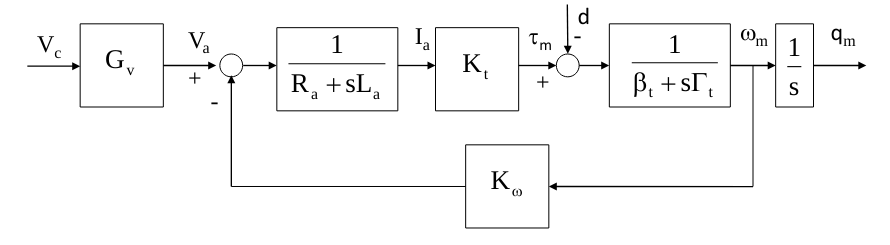
\includegraphics[width=0.7\linewidth]{images/decentralized_joint_space_control_3}
	\caption{Schema a blocchi del singolo giunto}
	\label{fig:decentralizedjointspacecontrol3}
\end{figure}


Cerchiamo ora di semplificare un po' questo modello. Possiamo iniziare supponendo $L_a$ trascurabile, dato che le perdite ad essa associate sono solitamente molto piccole.
Dall'equazione di equilibrio elettrico (\ref{eq:armature_balance}) possiamo quindi rimuovere $L_a$, e ottenere:
\begin{equation}\label{eq:simplified_armature_electrical_balance}
V_a - R_aI_a = K_\omega \omega_m
\end{equation}
Allora, ricordando che $I_a = \tau_m K_t^{-1}$ e sostituendo $\tau_m$ con l'espressione (\ref{eq:single_joint_dynamic_laplace}) otteniamo 
$$
V_a - R_a K_t^{-1} \tau_m = K_\omega \omega_m
\implies
V_a - R_a K_t^{-1} ((s\Gamma + \beta)\omega_m + d)
= K_\omega \omega_m
$$



Riorganizzando i termini, e ignorando il termine relativo a $\beta$ (visto che è trascurabile rispetto a $\omega_m$), otteniamo:
$$
\left( \frac{R_a \Gamma}{K_t K_\omega}s + 1 \right) \omega_m =
\frac{1}{K_\omega}V_a - \frac{R_a}{K_tK_\omega}d
$$

Da qui possiamo identificare 2 funzioni di trasferimento (a seconda di cosa consideriamo ingresso):

\begin{align}
G_\omega(s) &\triangleq \frac{\omega_m(s)}{V_a(s)} = \frac{1}{K_\omega(1 + sT)} \label{eq:tf_omega} \\
G_d(s) &\triangleq \frac{\omega_m(s)}{d(s)} = -\frac{T}{\Gamma(1 + sT)} = -K_dG_\omega(s)
\end{align}

dove:

$$
T = \frac{R_a \Gamma}{K_t K_\omega} 
\quad , \quad
K_d = \frac{R_a}{K_t}
$$

Da queste equazioni possiamo quindi passare allo schema a blocchi di fig. \ref{fig:decentralizedjointspacecontrol4}.

\begin{figure}[bh!]
	\centering
	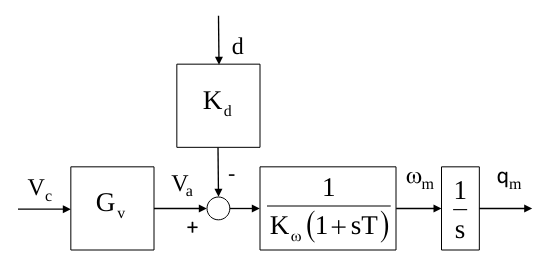
\includegraphics[width=0.6\linewidth]{images/decentralized_joint_space_control_4}
	\caption{Schema a blocchi semplificato}
	\label{fig:decentralizedjointspacecontrol4}
\end{figure}




\vspace*{20pt}
\begin{mdframed}[leftmargin=15pt, rightmargin=15pt, leftline=false, rightline=false]
\subsubsection{Comparazione con le slide di Rizzo}
\textit{Nelle slide è presente il seguente circuito. Anche se a prima vista potrebbe sembrare diverso è in realtà identico a quello di figura \ref{fig:decentralizedjointspacecontrol4}.}

{
	\centering
	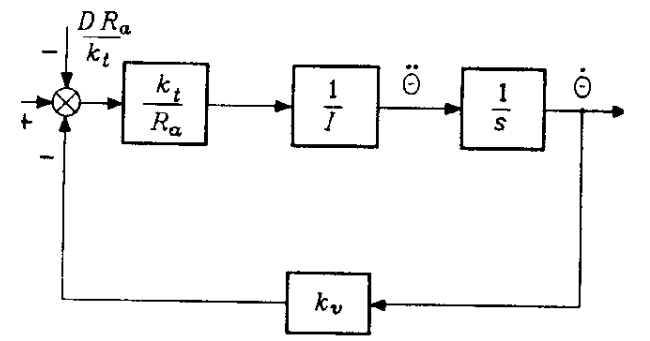
\includegraphics[width=0.6\linewidth]{images/decentralized_joint_space_control_5}
	\label{fig:decentralizedjointspacecontrol5}
	\par
}

\textit{Ricordando la differente notazione: $I \equiv \Gamma$, $k_v \equiv K_\omega$, possiamo unire i 3 blocchi in uno unico. Partiamo dal forward path:}
$$
F(s) = \frac{k_t}{R_a sI}
$$
\textit{Poi, incorporando il feedback, otteniamo}
$$
\frac{F(s)}{1 + F(s)k_v} = 
\frac{ \frac{k_t}{R_a sI} }{1 +  \frac{k_v k_t}{R_a sI} } = \frac{1}{k_v(1 + sT)}
$$

\textit{Ovvero la stessa forma di quanto mostrato in fig. \ref{fig:decentralizedjointspacecontrol4}.}
\end{mdframed}




\vspace{25pt}
\subsection{Struttura del controllo}

In fig. \ref{fig:decentralizedjointspacecontrol6} possiamo vedere lo schema di controllo generale, con retroazione su posizione, velocità e accelerazione (nota: per semplicità $G_v$ è stato incluso nell'anello di controllo più interno).

In generale, il controllore viene progettato modo che si abbia un guadagno elevato nel blocco a monte del punto di ingresso del disturbo (per ottenere un elevato fattore di attenuazione) e in modo che ci sia un’azione integrale, affinché gli effetti della coppia di gravità vengano cancellati in regime permanente.

\begin{figure}[H]
	\centering
	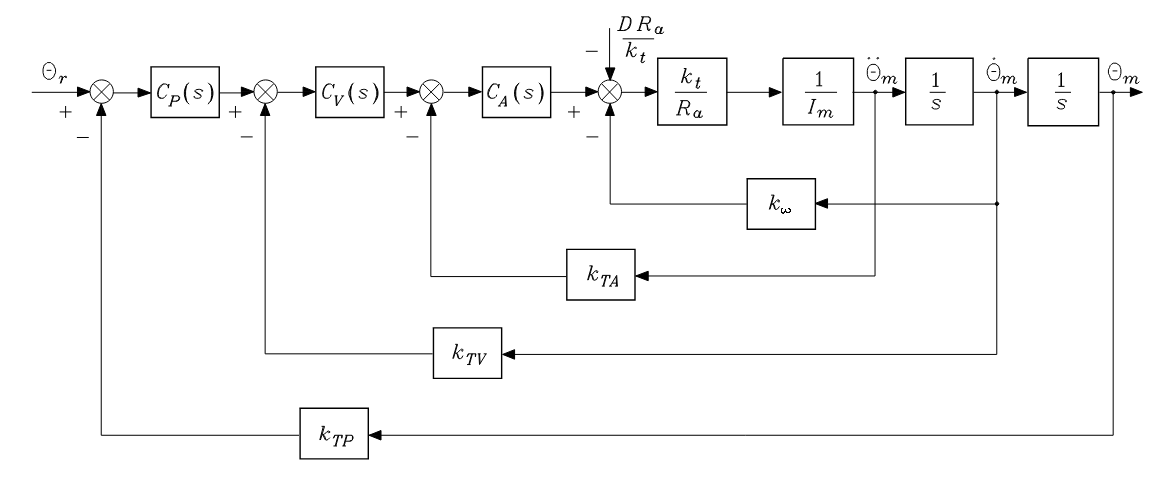
\includegraphics[width=0.9\linewidth]{images/decentralized_joint_space_control_6}
	\caption{Schema generale del controllo}
	\label{fig:decentralizedjointspacecontrol6}
\end{figure}


Queste richieste portano alla scelta di un \textbf{controllore PI (proporzionale-integrale)} della forma:
\begin{equation}\label{eq:pi_controller}
C(s) = K_p \frac{1+sT_p}{s}
\end{equation}






\subsubsection{Retroazione sulla posizione}
Possiamo partire dal caso più semplice, ovvero introducento un controllo con solo la retroazione $k_{TP}$ su $\theta_m$. Poniamo $C_v(s) = C_A(s) = 1$ e $k_{TV} = k_{TA} = 0$, mentre mettiamo $C_p(s)$ nella forma (\ref{eq:pi_controller}).

\begin{figure}[ht!]
	\centering
	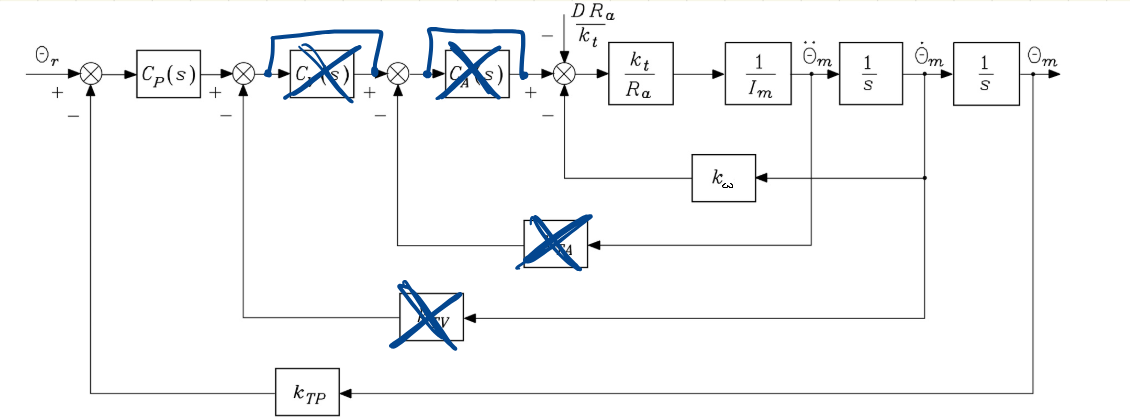
\includegraphics[width=0.7\linewidth]{images/position_feedback}
	\caption{Solo position feedback}
	\label{fig:positionfeedback}
\end{figure}

La funzione di trasferimento del ramo diretto risulta (richiamando (\ref{eq:pi_controller}) e (\ref{eq:tf_omega})):
$$
G(s) = 
\underbrace{C_p(s)}_{(\ref{eq:pi_controller})}
\underbrace{ \frac{1}{K_\omega(1 + sT)} }_{G_\omega(s) =(\ref{eq:tf_omega})}
\frac{1}{s}
= \frac{K_p(1+sT_p)}{s^2K_\omega(1+sT)}
$$
da cui si ricava la funzione di trasferimento ad anello chiuso:
$$
W(s) = \frac{K_p(1+sT_p)}{s^2K_\omega(1+sT) + K_P K_{TP} (1+sT_P)}
$$

Da qui è possibile analizzarne la stabilità, ad esempio tramite il luogo delle radici (vedi fig. \ref{fig:rootlocus1}).

\begin{figure}[ht!]
	\centering
	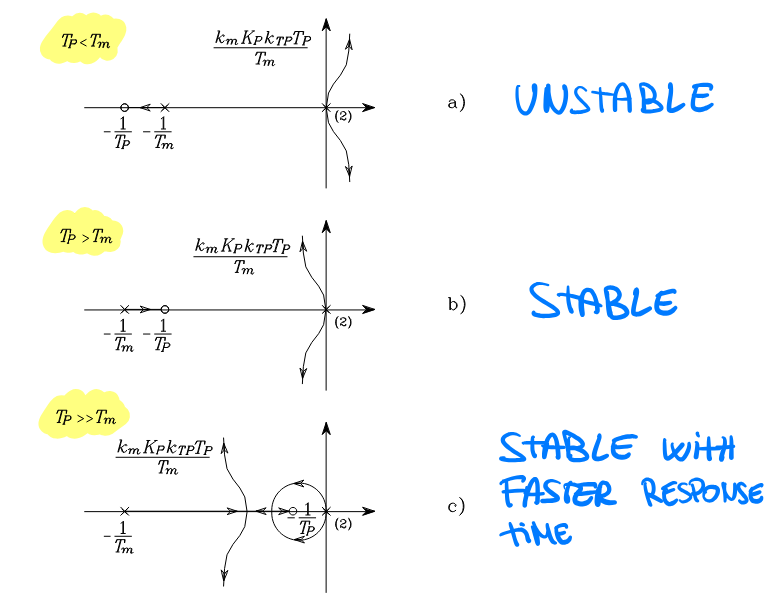
\includegraphics[width=0.7\linewidth]{images/root_locus_1}
	\caption{Root locus per $W(s)$ con solo retroazione sulla posizione}
	\label{fig:rootlocus1}
\end{figure}


I parametri $K_P$ e $T_P$ devono essere scelti in modo da:
\begin{itemize}
	\item Garantire l’asintotica stabilità del sistema in catena chiusa
	\item Evitare oscillazioni significative nella sua risposta
	\item Garantire un elevato fattore di attenuazione del disturbo 
\end{itemize}


Per calcolare meglio i requirements è possibile esprimere $W(s)$ in funzione di $\omega_n$ e $\zeta$:
$$
W(s) = \frac{\frac{1}{K_{TP}}(1+sT_P)}{\left( 1 + \frac{2\zeta}{\omega_n} + \frac{s^2}{\omega_n^2} \right) (1+\tau s) }
$$

Come possiamo vedere anche dal root locus:
\begin{itemize}
	\item Deve essere $T_P > T$ affinché si abbia asintotica stabilità
	\item Se $T_P \gg T$ si velocizza la risposta del sistema (diventano dominanti i poli complessi coniugati). Inoltre per elevati valori del guadagno $K_P$ la pulsazione del polo reale di $W(s)$ tende a quella dello zero ($\tau \approx T_P$) e quindi il sistema risulta rappresentato in prima approssimazione dalla sola dinamica del II° ordine associata ai poli complessi coniugati
	\item La parte reale dei poli dominanti non può comunque essere inferiore a $-1/(2T)$
\end{itemize}

Applicando le regole dell'algebra dei blocchi, è possibile anche ricavare la funzione di trasferimento fra il disturbo $D$ e l’uscita $\theta_m$ del sistema: $\Theta_m(s) / D(s)$.\\
Da questa t.f. è possibile vedere che \textbf{il fattore di attenuazione del disturbo vale} $\mathbf{K_PK_{TP}}$. Valori troppo elevati di $K_P$ possono però portare ad avere oscillazioni inaccettabili sull’uscita (lo smorzamento $\zeta$ risulta troppo piccolo).\\
Il tempo necessario per avere un’attenuazione significativa del disturbo è approssimabile come $T_R = max\{T_P, \frac{1}{\zeta \omega_n}\}$








\vspace{35pt}
\subsubsection{Retroazione di posizione e velocità}

Per questo secondo caso consideriamo il seguente setup (qua $C_A(s)=1$, $k_TA=0$):
$$
C_P(s) = K_P \qquad C_V(s)=K_V\frac{1+sT_V}{s}
$$
Ovvero un'azione solo proporzionale per la posizione, mentre un'azione PI per la velocità.

\begin{figure}[ht!]
	\centering
	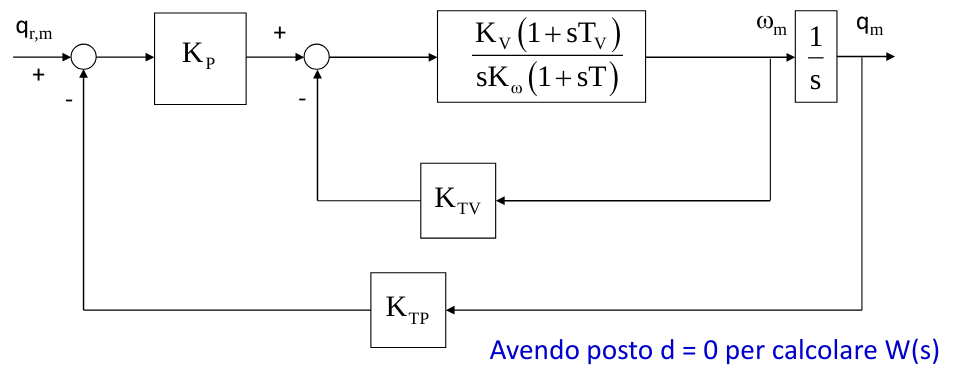
\includegraphics[width=0.7\linewidth]{images/decentralized_joint_space_control_7}
	\caption{Circuito con retroazione su posizione e velocità}
	\label{fig:decentralizedjointspacecontrol7}
\end{figure}


Di nuovo, possiamo analizzare la stabilità del sistema tramite il root-locus della funzione di trasferimento in ciclo chiuso $W(s)$ e gli effetti dei disturbi con la funzione di trasferimento $\Theta_m(s)/D(s)$.
$$
W(s)=\frac{K_P K_V}{K_\omega s^2 + K_V K_{TV} s + K_{TP} K_P K_V}
$$

Saltando nuovamente la forma esplicita di $\Theta_m(s)/D(s)$, possiamo dire che in questo caso il \textbf{fattore di attenuazione del disturbo} è dato dal prodotto $\mathbf{K_P K_{TV} K_V}$, ormai completamente definito, avendo imposto $K_P$ e $K_V$ per imporre i poli desiderati.

Aumentando il guadagno del feedback di posizione $K_P$, è possibile confinare i poli dell'anello chiuso in una regione del piano complesso con grandi valori assoluti della parte reale. Poi, la posizione effettiva può essere stabilita mediante una scelta adeguata di $K_V$.

\begin{figure}[!ht]
	\centering
	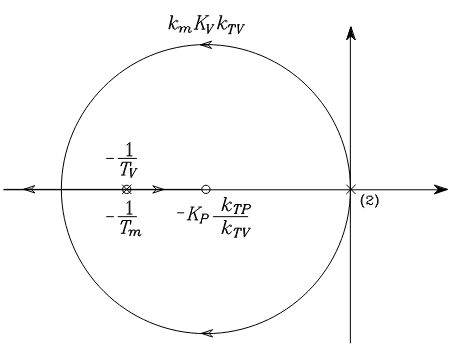
\includegraphics[width=0.5\linewidth]{images/root_locus_2}
	\caption{Root-locus con retroazione di velocità e posizione}
	\label{fig:rootlocus2}
\end{figure}







\vspace{35pt}
\subsubsection{Retroazione di posizione, velocità ed accelerazione}

Per concludere vediamo il controllo con tutti e 3 i feedback:
$$
C_P(s) = K_P \qquad C_V(s)=K_V \qquad C_A(s)=K_A\frac{1+sT_A}{s}
$$

Avendo a disposizione un parametro libero in più, sarebbe
possibile in questo caso:
\begin{itemize}
	\item Assegnare la dinamica desiderata al sistema ad anello chiuso
	\item Imporre il fattore di attenuazione del disturbo
\end{itemize}


\begin{figure}[ht!]
	\centering
	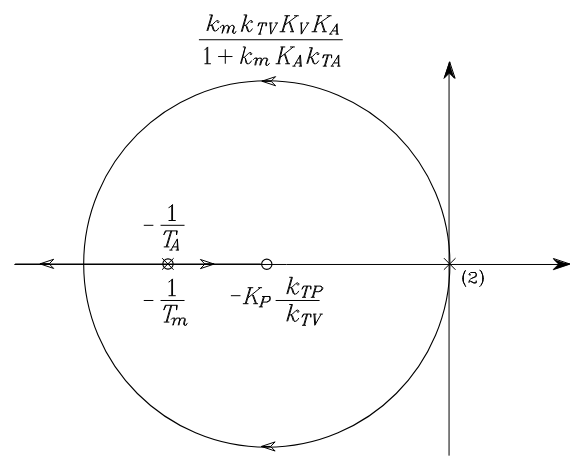
\includegraphics[width=0.5\linewidth]{images/root_locus_3}
	\caption{Root-locus con retroazione di accelerazione, velocità e posizione}
	\label{fig:rootlocus3}
\end{figure}

\textbf{Problema}:
La misura dell’\textbf{accelerazione però non è solitamente disponibile}. Per implementare uno schema di controllo comprendente la retroazione dell’accelerazione risulterebbe necessario ricavarla indirettamente dalle misure disponibili.

Avendo a disposizione la misura diretta della velocità, è possibile \textbf{stimare l’accelerazione} per mezzo di un filtro del primo ordine (vedi fig. \ref{fig:accelerationestimate}), purché avente banda sufficientemente ampia. Scegliendo questa larghezza di banda sufficientemente ampia, gli effetti dovuti ai ritardi di misurazione non sono un problema, e quindi è possibile prendere l'uscita del filtro di accelerazione come quantità per il feedback. Problemi possono comunque incorrere a causa del rumore presente sul segnale di accelerazione così ottenuto.

\begin{figure}[H]
	\centering
	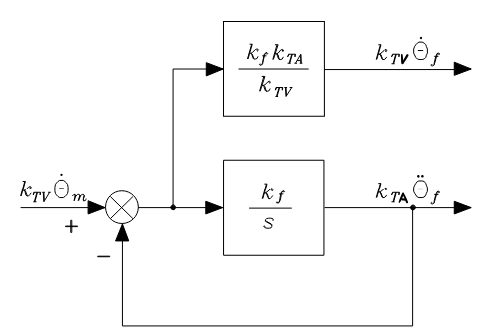
\includegraphics[width=0.4\linewidth]{images/acceleration_estimate}
	\caption{Filtro del I° ordine per la stima dell'accelerazione}
	\label{fig:accelerationestimate}
\end{figure}







\subsection{Attuatori saturanti}
In un’applicazione reale, il comportamento del sistema può allontanarsi da quello del suo modello teorico a causa di dinamiche “parassite” o non lineari, non incluse nella descrizione considerata, con evidenti conseguenze sulle prestazioni del controllo. Una di queste è ad esempio la presenza di attuatori saturanti.

Quest'ultima però può essere modellata semplicemente aggiugendo sul ramo diretto dell’anello di controllo un blocco che rappresenta la seguente relazione:
$$
\begin{cases}
	y_{max} & , \ u(t) > u_{max} \\
	ku(t) & , \ u_{min} \leq u(t) \leq u_{max} \\
	y_{min} & , \ u(t) < u_{min}
\end{cases}
$$


\begin{figure}[H]
	\centering
	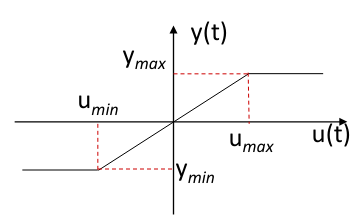
\includegraphics[width=0.4\linewidth]{images/saturation}
	\label{fig:saturation}
\end{figure}


L’inserimento di blocchi di \textbf{saturazione} è solitamente legato a \textbf{necessità di sicurezza e di salvaguardia} del sistema.

Quando le grandezze coinvolte (correnti, tensioni) raggiungono il valore massimo consentito ed entra in azione il blocco di saturazione, l’inseguimento della traiettoria non è più realizzato con le caratteristiche e l’accuratezza prevista. In caso di movimenti PTP non è inusuale che vengano raggiunte situazioni di saturazione: in tal caso infatti è solitamente prioritario raggiungere il più rapidamente possibile la configurazione finale desiderata, anziché rispettare la traiettoria prefissata in ogni istante.







\subsection{Feedforward compensation}
Quando è richiesto l’inseguimento di traiettorie con elevati valori di velocità e di accelerazione, è possibile ridurre l’errore di inseguimento utilizzando i valori del riferimento in velocità (ed in accelerazione) per calcolare termini di compensazione in avanti (feedforward compensation), da sommare all’azione del controllore posto sul ramo diretto.

Si noti che, in generale, calcolare derivate non è possibile (perchè dovremmo "predire il futuro"). In questo caso però essendo la traiettoria nota a priori, non ci sono problemi.

\begin{figure}[H]
	\centering
	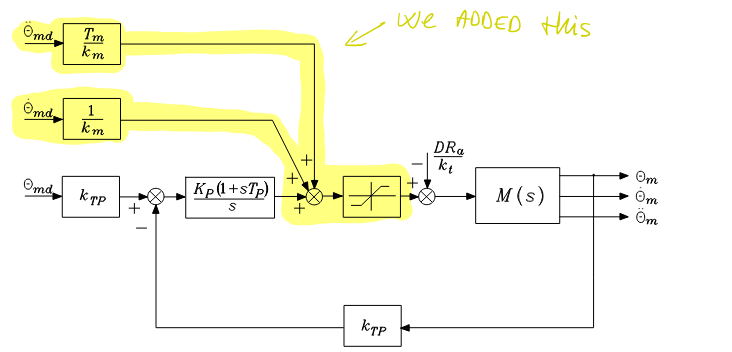
\includegraphics[width=0.7\linewidth]{images/feedforward_compensation}
	\caption{Schema a blocchi del controllo con feedback di posizione e feedforward compensation decentralizzato}
	\label{fig:feedforwardcompensation}
\end{figure}





\subsection{Computed torque	feedworward control}
È possibile aggiungere un altro blocco di feedforward.
Richiamando (\ref{eq:dynamic_with_disturbances}):
\boldmath
$$
K_r^{-1}\bar{B}K_r^{-1}\ddot{q}_m + F_m\dot{q}_m + d = \tau_m
$$
\unboldmath

se vogliamo reiettare perfettamente il disturbo $d$ potremmo provare a calcolarci in anticipo il valore di $d$, per poi sommarlo nel lato destro dell'equazione.

\boldmath
$$
K_r^{-1}\bar{B}K_r^{-1}\ddot{q}_m + F_m\dot{q}_m + \cancel{d} = \tau_m + \cancel{d}
$$
\unboldmath

Ponendo $q\equiv q_d$ ci basta usare (\ref{eq:dynamic_disturbances}) per calcolarci $d$ (offline).
 
\begin{figure}[H]
	\centering
	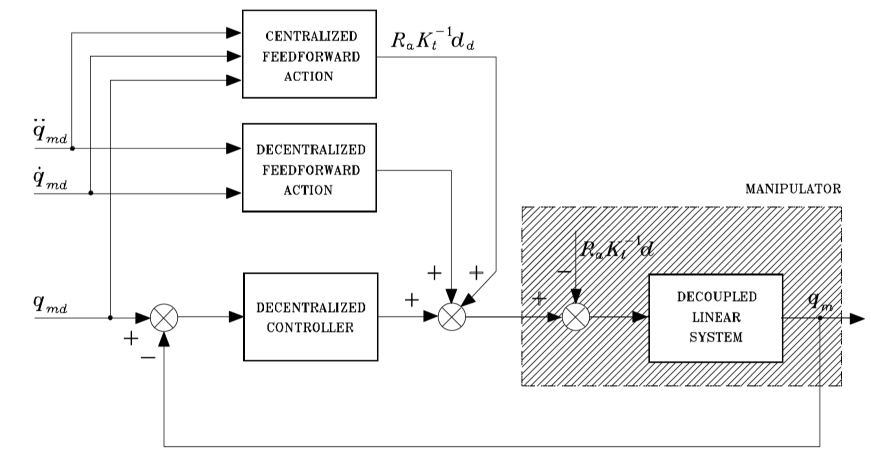
\includegraphics[width=0.7\linewidth]{images/computed_torque}
	\caption{Circuit with computed torque feedworward control}
	\label{fig:computedtorque}
\end{figure}



